\section{RA1}
\subsection*{Resultados de aprendizaje}
Identificar los elementos básicos desde el punto de vista del hardware y del software para analizar los principios de funcionamiento de las computadoras considerando una arquitectura genérica.

\subsection*{Contenido según programa}
Estructura de una computadora.  Antecedentes históricos.  Definición de unidades fundamentales (bit y byte) y sus múltiplos. Definición de memoria. Capacidad de memoria. Tipos de memoria. Buses. Unidad Central del Proceso (CPU).  Unidad Aritmética y Lógica (ALU). Unidad de Control.  Contador de Programa.  Dispositivos de entrada/salida (I/O).  Ejecución de instrucciones.  Fase de búsqueda de instrucciones. Secuencia de Instrucciones: Programa.  Conceptos de Hardware y Software. Interacción entre ambos elementos.


\subsection*{Estructura de una computadora}

\subsection{Ejercicios:}

\subsubsection{Clasifique los siguientes artículos como hardware o software:}
\begin{itemize}
  \item Procesador
  \item RAM
  \item Zinjai
  \item Preprocesador
  \item Impresora
  \item Explorador de Internet
\end{itemize}

\subsubsection{Raspberry pi}
La Raspberry Pi puede considerarse como una computadora portátil, un ordenador de placa única u ordenador de placa simple (SBC) de bajo coste desarrollado en el Reino Unido por la Raspberry Pi Foundation, con el objetivo de estimular la enseñanza de informática en las escuelas.
Busque en internet la información necesaria correspondiente al código de colores de una resistencia, y describa en no
mas de una hoja:
\begin{enumerate}[a)]
  \item Cuales son las diferentes versiones de la raspberry pi?
  \item Cuales son sus dimensiones y cuales son sus periféricos?
  \item Que sistema operativos puede utilizar?
  \item Mencionar un proyecto que pueda ser elaborado con esta placa.
\end{enumerate}

\begin{figure}[h!]
\centering
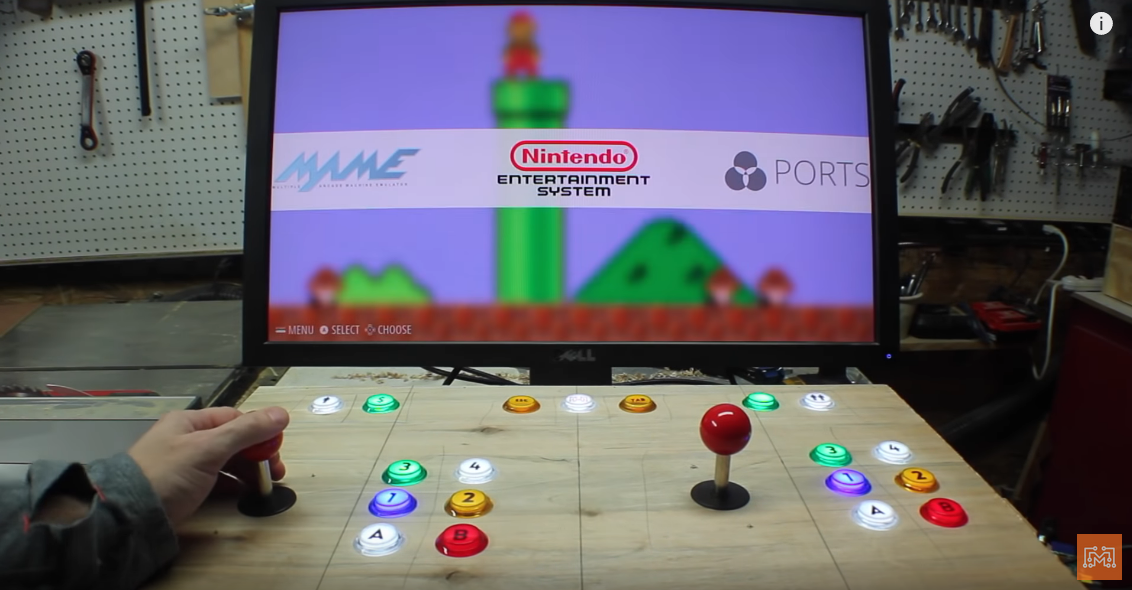
\includegraphics[width=.6\textwidth]{img/retropie.png}
\caption{Consola retropie realizada por ``I Like To Make Stuff''}
\label{fig:retropie}
\end{figure}
